\begin{verbatim}
"""
Created on Mon Apr 15 19:43:04 2019

Updated on Wed Jan 29 10:18:09 2020

@author: created by Sowmya Myneni and updated by Dijiang Huang
"""
\end{verbatim}

\begin{verbatim}
'\nCreated on Mon Apr 15 19:43:04 2019\n\nUpdated on Wed Jan 29 10:18:09 2020\n\n@author: created by Sowmya Myneni and updated by Dijiang Huang\n'
\end{verbatim}

\begin{verbatim}
import matplotlib.pyplot as plt
import tensorflow as tf
print("Num GPUs Available:", len(tf.config.list_physical_devices('GPU')))
\end{verbatim}

\begin{verbatim}
Num GPUs Available: 1
\end{verbatim}

\begin{verbatim}
import os
import multiprocessing

# Number of logical CPUs
num_cores = multiprocessing.cpu_count()
print(f"Number of CPU cores available: {num_cores}")
\end{verbatim}

\begin{verbatim}
Number of CPU cores available: 16
\end{verbatim}

\begin{verbatim}
# Configure TensorFlow to use all available CPU cores
#tf.config.threading.set_intra_op_parallelism_threads(0)  # Use all intra -operation threads
#tf.config.threading.set_inter_op_parallelism_threads(0)  # Use all inter -operation threads
\end{verbatim}

\paragraph{FNN Sample SA}

\begin{verbatim}
########################################
# Part 1 - Data Pre -Processing
#######################################

# To load a dataset file in Python, you can use Pandas. Import pandas using the line below
import pandas as pd
# Import numpy to perform operations on the dataset
import numpy as np
\end{verbatim}

\subparagraph{Variable Setup}

\begin{verbatim}
# Variable Setup
# Available datasets: KDDTrain+.txt, KDDTest+.txt, etc. More read Data Set Introduction.html within the NSL -KDD dataset folder
# Type the training dataset file name in ''
#TrainingDataPath='NSL -KDD/'
#TrainingData='KDDTrain+_20Percent.txt'
# Batch Size
BatchSize=10
# Epohe Size
NumEpoch=10
\end{verbatim}

\subparagraph{Import Training Dataset}

\begin{verbatim}
# Import dataset.
# Dataset is given in TraningData variable You can replace it with the file 
# path such as “C:\Users\...\dataset.csv’. 
# The file can be a .txt as well. 
# If the dataset file has header, then keep header=0 otherwise use header=none
# reference: https://www.shanelynn.ie/select -pandas -dataframe -rows -and -columns -using -iloc -loc -and -ix/
dataset_train = pd.read_csv('Training -a1 -a3.csv', header=None)
\end{verbatim}

\begin{verbatim}
dataset_train.info()
\end{verbatim}

\begin{verbatim}
<class 'pandas.core.frame.DataFrame'>
RangeIndex: 113322 entries, 0 to 113321
Data columns (total 43 columns):
 #   Column  Non -Null Count   Dtype  
 - - -  - - - - - -  - - - - - - - - - - - - - -   - - - - -  
 0   0       113322 non -null  int64  
 1   1       113322 non -null  object 
 2   2       113322 non -null  object 
 3   3       113322 non -null  object 
 4   4       113322 non -null  int64  
 5   5       113322 non -null  int64  
 6   6       113322 non -null  int64  
 7   7       113322 non -null  int64  
 8   8       113322 non -null  int64  
 9   9       113322 non -null  int64  
 10  10      113322 non -null  int64  
 11  11      113322 non -null  int64  
 12  12      113322 non -null  int64  
 13  13      113322 non -null  int64  
 14  14      113322 non -null  int64  
 15  15      113322 non -null  int64  
 16  16      113322 non -null  int64  
 17  17      113322 non -null  int64  
 18  18      113322 non -null  int64  
 19  19      113322 non -null  int64  
 20  20      113322 non -null  int64  
 21  21      113322 non -null  int64  
 22  22      113322 non -null  int64  
 23  23      113322 non -null  int64  
 24  24      113322 non -null  float64
 25  25      113322 non -null  float64
 26  26      113322 non -null  float64
 27  27      113322 non -null  float64
 28  28      113322 non -null  float64
 29  29      113322 non -null  float64
 30  30      113322 non -null  float64
 31  31      113322 non -null  int64  
 32  32      113322 non -null  int64  
 33  33      113322 non -null  float64
 34  34      113322 non -null  float64
 35  35      113322 non -null  float64
 36  36      113322 non -null  float64
 37  37      113322 non -null  float64
 38  38      113322 non -null  float64
 39  39      113322 non -null  float64
 40  40      113322 non -null  float64
 41  41      113322 non -null  object 
 42  42      113322 non -null  int64  
dtypes: float64(15), int64(24), object(4)
memory usage: 37.2+ MB
\end{verbatim}

\begin{verbatim}
dataset_train.describe()
\end{verbatim}

\bigskip\noindent
\begin{tabular}{p{\dimexpr 0.045\linewidth-2\tabcolsep}p{\dimexpr 0.045\linewidth-2\tabcolsep}p{\dimexpr 0.045\linewidth-2\tabcolsep}p{\dimexpr 0.045\linewidth-2\tabcolsep}p{\dimexpr 0.045\linewidth-2\tabcolsep}p{\dimexpr 0.045\linewidth-2\tabcolsep}p{\dimexpr 0.045\linewidth-2\tabcolsep}p{\dimexpr 0.045\linewidth-2\tabcolsep}p{\dimexpr 0.045\linewidth-2\tabcolsep}p{\dimexpr 0.045\linewidth-2\tabcolsep}p{\dimexpr 0.045\linewidth-2\tabcolsep}p{\dimexpr 0.045\linewidth-2\tabcolsep}p{\dimexpr 0.045\linewidth-2\tabcolsep}p{\dimexpr 0.045\linewidth-2\tabcolsep}p{\dimexpr 0.045\linewidth-2\tabcolsep}p{\dimexpr 0.045\linewidth-2\tabcolsep}p{\dimexpr 0.045\linewidth-2\tabcolsep}p{\dimexpr 0.045\linewidth-2\tabcolsep}p{\dimexpr 0.045\linewidth-2\tabcolsep}p{\dimexpr 0.045\linewidth-2\tabcolsep}p{\dimexpr 0.045\linewidth-2\tabcolsep}p{\dimexpr 0.045\linewidth-2\tabcolsep}}
\toprule
 & 0 & 4 & 5 & 6 & 7 & 8 & 9 & 10 & 11 & 12 & ... & 32 & 33 & 34 & 35 & 36 & 37 & 38 & 39 & 40 & 42 \\
\hline
count & 113322.000000 & 1.133220e+05 & 1.133220e+05 & 113322.000000 & 113322.000000 & 113322.000000 & 113322.00000 & 113322.000000 & 113322.000000 & 113322.000000 & ... & 113322.000000 & 113322.000000 & 113322.000000 & 113322.000000 & 113322.000000 & 113322.000000 & 113322.000000 & 113322.000000 & 113322.000000 & 113322.000000 \\
\hline
mean & 100.224811 & 8.281767e+03 & 2.643902e+03 & 0.000221 & 0.025220 & 0.000097 & 0.15388 & 0.000829 & 0.431161 & 0.309684 & ... & 123.833819 & 0.532846 & 0.050752 & 0.092656 & 0.016153 & 0.311395 & 0.305340 & 0.091564 & 0.087884 & 19.901573 \\
\hline
std & 1008.980950 & 3.224064e+05 & 5.051136e+04 & 0.014851 & 0.267188 & 0.013613 & 1.79114 & 0.038265 & 0.495241 & 25.242551 & ... & 111.849033 & 0.444796 & 0.106580 & 0.233168 & 0.057117 & 0.458715 & 0.458058 & 0.279031 & 0.276273 & 1.717580 \\
\hline
min & 0.000000 & 0.000000e+00 & 0.000000e+00 & 0.000000 & 0.000000 & 0.000000 & 0.00000 & 0.000000 & 0.000000 & 0.000000 & ... & 0.000000 & 0.000000 & 0.000000 & 0.000000 & 0.000000 & 0.000000 & 0.000000 & 0.000000 & 0.000000 & 0.000000 \\
\hline
25\% & 0.000000 & 0.000000e+00 & 0.000000e+00 & 0.000000 & 0.000000 & 0.000000 & 0.00000 & 0.000000 & 0.000000 & 0.000000 & ... & 13.000000 & 0.050000 & 0.000000 & 0.000000 & 0.000000 & 0.000000 & 0.000000 & 0.000000 & 0.000000 & 19.000000 \\
\hline
50\% & 0.000000 & 5.900000e+01 & 3.600000e+01 & 0.000000 & 0.000000 & 0.000000 & 0.00000 & 0.000000 & 0.000000 & 0.000000 & ... & 83.000000 & 0.580000 & 0.020000 & 0.000000 & 0.000000 & 0.000000 & 0.000000 & 0.000000 & 0.000000 & 21.000000 \\
\hline
75\% & 0.000000 & 2.900000e+02 & 7.610000e+02 & 0.000000 & 0.000000 & 0.000000 & 0.00000 & 0.000000 & 1.000000 & 0.000000 & ... & 255.000000 & 1.000000 & 0.070000 & 0.030000 & 0.010000 & 1.000000 & 1.000000 & 0.000000 & 0.000000 & 21.000000 \\
\hline
max & 40504.000000 & 8.958152e+07 & 7.028652e+06 & 1.000000 & 3.000000 & 3.000000 & 77.00000 & 4.000000 & 1.000000 & 7479.000000 & ... & 255.000000 & 1.000000 & 1.000000 & 1.000000 & 1.000000 & 1.000000 & 1.000000 & 1.000000 & 1.000000 & 21.000000 \\
\hline
\bottomrule
\end{tabular}

\bigskip

8 rows $\times$ 39 columns

\begin{verbatim}
# Identify the column that contains the attack types
# Assuming the column with attack types is named based on the sample data ("neptune", "normal", etc.)
attack_column = dataset_train.columns[ -2]  # Second last column seems to have attack types

# Calculate the frequency of each attack type
attack_distribution = dataset_train[attack_column].value_counts()

plt.figure(figsize=(10, 6))
attack_distribution.plot(kind='bar', logy=True)
plt.title('A1 and A3 Training Dataset Distribution of Attack Types')
plt.xlabel('Attack Type')
plt.ylabel('Frequency')
plt.xticks(rotation=45)
plt.tight_layout()
plt.show()
\end{verbatim}

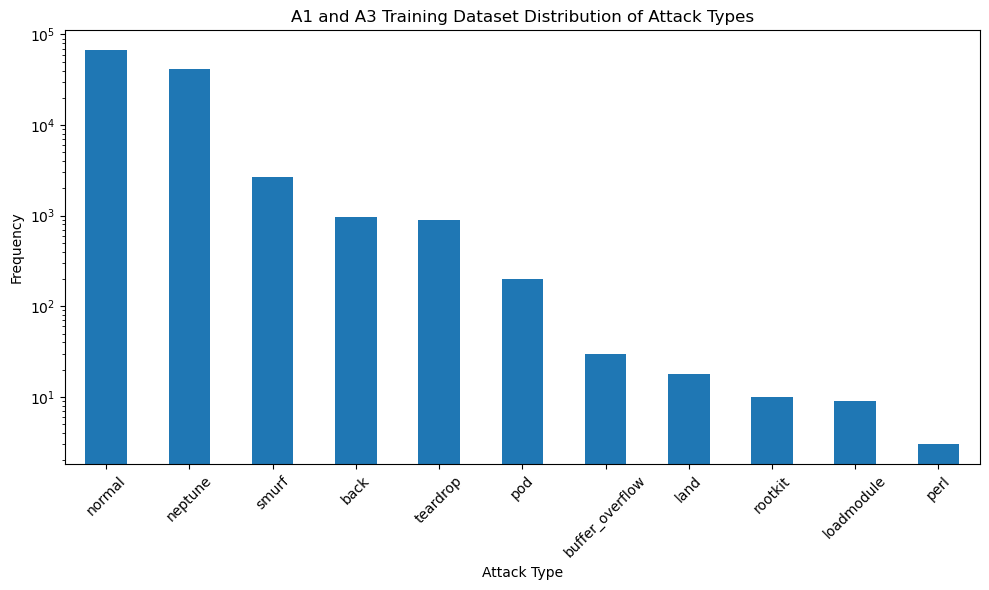
\includegraphics[width=0.7\linewidth]{files/6e5ff7af9c74632a0481808420b94337.png}

\begin{verbatim}
X_train = dataset_train.iloc[:, 0: -2].values
X_train
\end{verbatim}

\begin{verbatim}
array([[0, 'tcp', 'ftp_data', ..., 0.0, 0.05, 0.0],
       [0, 'udp', 'other', ..., 0.0, 0.0, 0.0],
       [0, 'tcp', 'private', ..., 1.0, 0.0, 0.0],
       ...,
       [0, 'tcp', 'smtp', ..., 0.0, 0.01, 0.0],
       [0, 'tcp', 'klogin', ..., 1.0, 0.0, 0.0],
       [0, 'tcp', 'ftp_data', ..., 0.0, 0.0, 0.0]], dtype=object)
\end{verbatim}

\begin{verbatim}
X_train.shape
\end{verbatim}

\begin{verbatim}
(113322, 41)
\end{verbatim}

\begin{verbatim}
label_column_train = dataset_train.iloc[:, -2].values
label_column_train
\end{verbatim}

\begin{verbatim}
array(['normal', 'normal', 'neptune', ..., 'normal', 'neptune', 'normal'],
      dtype=object)
\end{verbatim}

\begin{verbatim}
y_train = []
for i in range(len(label_column_train)):
    if label_column_train[i] == 'normal':
        y_train.append(0)
    else:
        y_train.append(1)

# Convert list to array
y_train = np.array(y_train)
\end{verbatim}

\begin{verbatim}
y_train
\end{verbatim}

\begin{verbatim}
array([0, 0, 1, ..., 0, 1, 0])
\end{verbatim}

\begin{verbatim}
y_train.shape
\end{verbatim}

\begin{verbatim}
(113322,)
\end{verbatim}

\subparagraph{Import Testing Dataset}

\begin{verbatim}
# Import dataset.
# Dataset is given in TraningData variable You can replace it with the file 
# path such as “C:\Users\...\dataset.csv’. 
# The file can be a .txt as well. 
# If the dataset file has header, then keep header=0 otherwise use header=none
# reference: https://www.shanelynn.ie/select -pandas -dataframe -rows -and -columns -using -iloc -loc -and -ix/
dataset_test = pd.read_csv('Testing -a2 -a4.csv', header=None)
\end{verbatim}

\begin{verbatim}
dataset_test.info()
\end{verbatim}

\begin{verbatim}
<class 'pandas.core.frame.DataFrame'>
RangeIndex: 15017 entries, 0 to 15016
Data columns (total 43 columns):
 #   Column  Non -Null Count  Dtype  
 - - -  - - - - - -  - - - - - - - - - - - - - -  - - - - -  
 0   0       15017 non -null  int64  
 1   1       15017 non -null  object 
 2   2       15017 non -null  object 
 3   3       15017 non -null  object 
 4   4       15017 non -null  int64  
 5   5       15017 non -null  int64  
 6   6       15017 non -null  int64  
 7   7       15017 non -null  int64  
 8   8       15017 non -null  int64  
 9   9       15017 non -null  int64  
 10  10      15017 non -null  int64  
 11  11      15017 non -null  int64  
 12  12      15017 non -null  int64  
 13  13      15017 non -null  int64  
 14  14      15017 non -null  int64  
 15  15      15017 non -null  int64  
 16  16      15017 non -null  int64  
 17  17      15017 non -null  int64  
 18  18      15017 non -null  int64  
 19  19      15017 non -null  int64  
 20  20      15017 non -null  int64  
 21  21      15017 non -null  int64  
 22  22      15017 non -null  int64  
 23  23      15017 non -null  int64  
 24  24      15017 non -null  float64
 25  25      15017 non -null  float64
 26  26      15017 non -null  float64
 27  27      15017 non -null  float64
 28  28      15017 non -null  float64
 29  29      15017 non -null  float64
 30  30      15017 non -null  float64
 31  31      15017 non -null  int64  
 32  32      15017 non -null  int64  
 33  33      15017 non -null  float64
 34  34      15017 non -null  float64
 35  35      15017 non -null  float64
 36  36      15017 non -null  float64
 37  37      15017 non -null  float64
 38  38      15017 non -null  float64
 39  39      15017 non -null  float64
 40  40      15017 non -null  float64
 41  41      15017 non -null  object 
 42  42      15017 non -null  int64  
dtypes: float64(15), int64(24), object(4)
memory usage: 4.9+ MB
\end{verbatim}

\begin{verbatim}
dataset_test.describe()
\end{verbatim}

\bigskip\noindent
\begin{tabular}{p{\dimexpr 0.045\linewidth-2\tabcolsep}p{\dimexpr 0.045\linewidth-2\tabcolsep}p{\dimexpr 0.045\linewidth-2\tabcolsep}p{\dimexpr 0.045\linewidth-2\tabcolsep}p{\dimexpr 0.045\linewidth-2\tabcolsep}p{\dimexpr 0.045\linewidth-2\tabcolsep}p{\dimexpr 0.045\linewidth-2\tabcolsep}p{\dimexpr 0.045\linewidth-2\tabcolsep}p{\dimexpr 0.045\linewidth-2\tabcolsep}p{\dimexpr 0.045\linewidth-2\tabcolsep}p{\dimexpr 0.045\linewidth-2\tabcolsep}p{\dimexpr 0.045\linewidth-2\tabcolsep}p{\dimexpr 0.045\linewidth-2\tabcolsep}p{\dimexpr 0.045\linewidth-2\tabcolsep}p{\dimexpr 0.045\linewidth-2\tabcolsep}p{\dimexpr 0.045\linewidth-2\tabcolsep}p{\dimexpr 0.045\linewidth-2\tabcolsep}p{\dimexpr 0.045\linewidth-2\tabcolsep}p{\dimexpr 0.045\linewidth-2\tabcolsep}p{\dimexpr 0.045\linewidth-2\tabcolsep}p{\dimexpr 0.045\linewidth-2\tabcolsep}p{\dimexpr 0.045\linewidth-2\tabcolsep}}
\toprule
 & 0 & 4 & 5 & 6 & 7 & 8 & 9 & 10 & 11 & 12 & ... & 32 & 33 & 34 & 35 & 36 & 37 & 38 & 39 & 40 & 42 \\
\hline
count & 15017.000000 & 1.501700e+04 & 1.501700e+04 & 15017.0 & 15017.000000 & 15017.000000 & 15017.000000 & 15017.000000 & 15017.000000 & 15017.000000 & ... & 15017.000000 & 15017.000000 & 15017.000000 & 15017.000000 & 15017.000000 & 15017.00000 & 15017.000000 & 15017.000000 & 15017.000000 & 15017.000000 \\
\hline
mean & 49.544916 & 1.226061e+04 & 2.840014e+03 & 0.0 & 0.008390 & 0.000067 & 0.104948 & 0.032297 & 0.584138 & 0.124858 & ... & 169.158088 & 0.742390 & 0.100937 & 0.154092 & 0.027942 & 0.02463 & 0.021677 & 0.102269 & 0.108134 & 17.781448 \\
\hline
std & 1071.012267 & 5.791198e+05 & 2.585708e+04 & 0.0 & 0.152003 & 0.008160 & 1.081785 & 0.182721 & 0.492886 & 8.760658 & ... & 104.665702 & 0.382547 & 0.258687 & 0.317539 & 0.098983 & 0.13561 & 0.139979 & 0.263894 & 0.296870 & 4.672454 \\
\hline
min & 0.000000 & 0.000000e+00 & 0.000000e+00 & 0.0 & 0.000000 & 0.000000 & 0.000000 & 0.000000 & 0.000000 & 0.000000 & ... & 0.000000 & 0.000000 & 0.000000 & 0.000000 & 0.000000 & 0.00000 & 0.000000 & 0.000000 & 0.000000 & 0.000000 \\
\hline
25\% & 0.000000 & 3.000000e+01 & 3.600000e+01 & 0.0 & 0.000000 & 0.000000 & 0.000000 & 0.000000 & 0.000000 & 0.000000 & ... & 53.000000 & 0.390000 & 0.000000 & 0.000000 & 0.000000 & 0.00000 & 0.000000 & 0.000000 & 0.000000 & 16.000000 \\
\hline
50\% & 0.000000 & 1.890000e+02 & 2.760000e+02 & 0.0 & 0.000000 & 0.000000 & 0.000000 & 0.000000 & 1.000000 & 0.000000 & ... & 250.000000 & 1.000000 & 0.000000 & 0.010000 & 0.000000 & 0.00000 & 0.000000 & 0.000000 & 0.000000 & 21.000000 \\
\hline
75\% & 0.000000 & 2.870000e+02 & 1.399000e+03 & 0.0 & 0.000000 & 0.000000 & 0.000000 & 0.000000 & 1.000000 & 0.000000 & ... & 255.000000 & 1.000000 & 0.030000 & 0.060000 & 0.020000 & 0.00000 & 0.000000 & 0.010000 & 0.000000 & 21.000000 \\
\hline
max & 57715.000000 & 6.282565e+07 & 1.345927e+06 & 0.0 & 3.000000 & 1.000000 & 101.000000 & 4.000000 & 1.000000 & 796.000000 & ... & 255.000000 & 1.000000 & 1.000000 & 1.000000 & 1.000000 & 1.00000 & 1.000000 & 1.000000 & 1.000000 & 21.000000 \\
\hline
\bottomrule
\end{tabular}

\bigskip

8 rows $\times$ 39 columns

\begin{verbatim}
# Identify the column that contains the attack types
# Assuming the column with attack types is named based on the sample data ("neptune", "normal", etc.)
attack_column = dataset_test.columns[ -2]  # Second last column seems to have attack types

# Calculate the frequency of each attack type
attack_distribution = dataset_test[attack_column].value_counts()

plt.figure(figsize=(10, 6))
attack_distribution.plot(kind='bar', logy=True)
plt.title('A2 and A4 Testing Dataset Distribution of Attack Types')
plt.xlabel('Attack Type')
plt.ylabel('Frequency')
plt.xticks(rotation=45)
plt.tight_layout()
plt.show()
\end{verbatim}

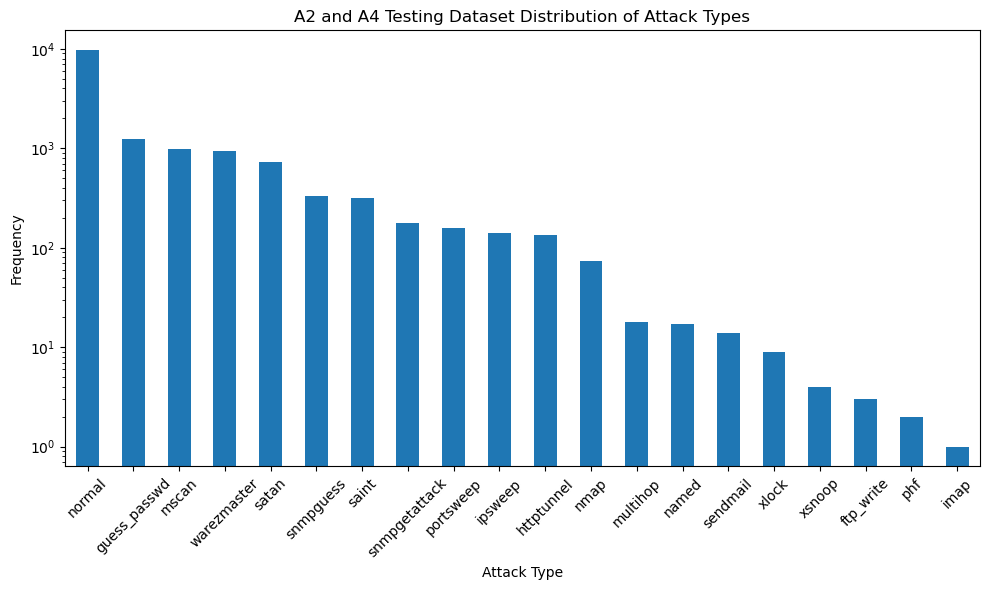
\includegraphics[width=0.7\linewidth]{files/22e3f668b599233b74804f180141e239.png}

\begin{verbatim}
X_test = dataset_test.iloc[:, 0: -2].values
X_test
\end{verbatim}

\begin{verbatim}
array([[2, 'tcp', 'ftp_data', ..., 0.0, 0.0, 0.0],
       [0, 'icmp', 'eco_i', ..., 0.0, 0.0, 0.0],
       [1, 'tcp', 'telnet', ..., 0.0, 0.83, 0.71],
       ...,
       [0, 'tcp', 'http', ..., 0.0, 0.0, 0.0],
       [0, 'udp', 'domain_u', ..., 0.0, 0.0, 0.0],
       [0, 'tcp', 'sunrpc', ..., 0.0, 0.44, 1.0]], dtype=object)
\end{verbatim}

\begin{verbatim}
X_test.shape
\end{verbatim}

\begin{verbatim}
(15017, 41)
\end{verbatim}

\begin{verbatim}
label_column_test = dataset_test.iloc[:, -2].values
label_column_test
\end{verbatim}

\begin{verbatim}
array(['normal', 'saint', 'mscan', ..., 'normal', 'normal', 'mscan'],
      dtype=object)
\end{verbatim}

\begin{verbatim}
y_test = []
for i in range(len(label_column_test)):
    if label_column_test[i] == 'normal':
        y_test.append(0)
    else:
        y_test.append(1)

# Convert list to array
y_test = np.array(y_test)
\end{verbatim}

\begin{verbatim}
y_test
\end{verbatim}

\begin{verbatim}
array([0, 1, 1, ..., 0, 0, 1])
\end{verbatim}

\subparagraph{Encoding categorical data (convert letters/words in numbers)}

\begin{verbatim}
# The following code work Python 3.7 or newer
from sklearn.preprocessing import OneHotEncoder
from sklearn.compose import ColumnTransformer
ct = ColumnTransformer(
     # The column numbers to be transformed ([1, 2, 3] represents three columns to be transferred)
    [('one_hot_encoder', OneHotEncoder(handle_unknown='ignore'), [1,2,3])],
    # Leave the rest of the columns untouched
    remainder='passthrough'
)
X_train = np.array(ct.fit_transform(X_train), dtype=np.float64)
X_test  = np.array(ct.transform(X_test) , dtype=np.float64)
\end{verbatim}

\begin{verbatim}
X_train
\end{verbatim}

\begin{verbatim}
array([[0.  , 1.  , 0.  , ..., 0.  , 0.05, 0.  ],
       [0.  , 0.  , 1.  , ..., 0.  , 0.  , 0.  ],
       [0.  , 1.  , 0.  , ..., 1.  , 0.  , 0.  ],
       ...,
       [0.  , 1.  , 0.  , ..., 0.  , 0.01, 0.  ],
       [0.  , 1.  , 0.  , ..., 1.  , 0.  , 0.  ],
       [0.  , 1.  , 0.  , ..., 0.  , 0.  , 0.  ]])
\end{verbatim}

\begin{verbatim}
X_train[0]
\end{verbatim}

\begin{verbatim}
array([0.00e+00, 1.00e+00, 0.00e+00, 0.00e+00, 0.00e+00, 0.00e+00,
       0.00e+00, 0.00e+00, 0.00e+00, 0.00e+00, 0.00e+00, 0.00e+00,
       0.00e+00, 0.00e+00, 0.00e+00, 0.00e+00, 0.00e+00, 0.00e+00,
       0.00e+00, 0.00e+00, 0.00e+00, 0.00e+00, 1.00e+00, 0.00e+00,
       0.00e+00, 0.00e+00, 0.00e+00, 0.00e+00, 0.00e+00, 0.00e+00,
       0.00e+00, 0.00e+00, 0.00e+00, 0.00e+00, 0.00e+00, 0.00e+00,
       0.00e+00, 0.00e+00, 0.00e+00, 0.00e+00, 0.00e+00, 0.00e+00,
       0.00e+00, 0.00e+00, 0.00e+00, 0.00e+00, 0.00e+00, 0.00e+00,
       0.00e+00, 0.00e+00, 0.00e+00, 0.00e+00, 0.00e+00, 0.00e+00,
       0.00e+00, 0.00e+00, 0.00e+00, 0.00e+00, 0.00e+00, 0.00e+00,
       0.00e+00, 0.00e+00, 0.00e+00, 0.00e+00, 0.00e+00, 0.00e+00,
       0.00e+00, 0.00e+00, 0.00e+00, 0.00e+00, 0.00e+00, 0.00e+00,
       0.00e+00, 0.00e+00, 0.00e+00, 0.00e+00, 1.00e+00, 0.00e+00,
       0.00e+00, 4.91e+02, 0.00e+00, 0.00e+00, 0.00e+00, 0.00e+00,
       0.00e+00, 0.00e+00, 0.00e+00, 0.00e+00, 0.00e+00, 0.00e+00,
       0.00e+00, 0.00e+00, 0.00e+00, 0.00e+00, 0.00e+00, 0.00e+00,
       0.00e+00, 2.00e+00, 2.00e+00, 0.00e+00, 0.00e+00, 0.00e+00,
       0.00e+00, 1.00e+00, 0.00e+00, 0.00e+00, 1.50e+02, 2.50e+01,
       1.70e -01, 3.00e -02, 1.70e -01, 0.00e+00, 0.00e+00, 0.00e+00,
       5.00e -02, 0.00e+00])
\end{verbatim}

\begin{verbatim}
X_train.shape
\end{verbatim}

\begin{verbatim}
(113322, 116)
\end{verbatim}

\begin{verbatim}
X_test
\end{verbatim}

\begin{verbatim}
array([[0.  , 1.  , 0.  , ..., 0.  , 0.  , 0.  ],
       [1.  , 0.  , 0.  , ..., 0.  , 0.  , 0.  ],
       [0.  , 1.  , 0.  , ..., 0.  , 0.83, 0.71],
       ...,
       [0.  , 1.  , 0.  , ..., 0.  , 0.  , 0.  ],
       [0.  , 0.  , 1.  , ..., 0.  , 0.  , 0.  ],
       [0.  , 1.  , 0.  , ..., 0.  , 0.44, 1.  ]])
\end{verbatim}

\begin{verbatim}
X_test.shape
\end{verbatim}

\begin{verbatim}
(15017, 116)
\end{verbatim}

\subparagraph{Perform feature scaling}

\begin{verbatim}
# Perform feature scaling. For ANN you can use StandardScaler, for RNNs recommended is 
# MinMaxScaler. 
# referece: https://scikit -learn.org/stable/modules/generated/sklearn.preprocessing.StandardScaler.html
# https://scikit -learn.org/stable/modules/preprocessing.html
from sklearn.preprocessing import StandardScaler
sc = StandardScaler()
X_train = sc.fit_transform(X_train)  # Scaling to the range [0,1]
X_test  = sc.fit_transform(X_test)
\end{verbatim}

\begin{verbatim}
X_train
\end{verbatim}

\begin{verbatim}
array([[ -0.19511653,  0.42713604, -0.36510181, ..., -0.66659951,
        -0.14895839, -0.31810766],
       [ -0.19511653, -2.34117451,  2.73896205, ..., -0.66659951,
        -0.32815058, -0.31810766],
       [ -0.19511653,  0.42713604, -0.36510181, ...,  1.51653833,
        -0.32815058, -0.31810766],
       ...,
       [ -0.19511653,  0.42713604, -0.36510181, ..., -0.66659951,
        -0.29231215, -0.31810766],
       [ -0.19511653,  0.42713604, -0.36510181, ...,  1.51653833,
        -0.32815058, -0.31810766],
       [ -0.19511653,  0.42713604, -0.36510181, ..., -0.66659951,
        -0.32815058, -0.31810766]])
\end{verbatim}

\begin{verbatim}
y_train
\end{verbatim}

\begin{verbatim}
array([0, 0, 1, ..., 0, 1, 0])
\end{verbatim}

\paragraph{Part 2: Building FNN}

\begin{verbatim}
########################################
# Part 2: Building FNN
#######################################

# Importing the Keras libraries and packages
import keras
from keras.models import Sequential
from keras.layers import Dense, Input
\end{verbatim}

\subparagraph{Initializing the ANN}

\begin{verbatim}
# Initialising the ANN
# Reference: https://machinelearningmastery.com/tutorial -first -neural -network -python -keras/
classifier = Sequential()
classifier
\end{verbatim}

\begin{verbatim}
<keras.engine.sequential.Sequential at 0x19cb8de02e0>
\end{verbatim}

\subparagraph{Adding the input layer and the first hidden layer, 6 nodes, input\_dim specifies the number of variables}

\begin{verbatim}
# Adding the input layer and the first hidden layer, 6 nodes, input_dim specifies the number of variables
# rectified linear unit activation function relu, reference: https://machinelearningmastery.com/rectified -linear -activation -function -for -deep -learning -neural -networks/
# Adding the input layer with Input() and the first hidden layer
classifier.add(Input(shape=(len(X_train[0]),)))  # Input layer
classifier.add(Dense(units=6, kernel_initializer='uniform', activation='relu'))

# Adding the second hidden layer
classifier.add(Dense(units=6, kernel_initializer='uniform', activation='relu'))

# Adding the output layer
classifier.add(Dense(units=1, kernel_initializer='uniform', activation='sigmoid'))
\end{verbatim}

\subparagraph{Compiling the ANN}

\begin{verbatim}
# Compiling the ANN, 

# Gradient descent algorithm “adam“, Reference: https://machinelearningmastery.com/adam -optimization -algorithm -for -deep -learning/

# This loss is for a binary classification problems and is defined in Keras as “binary_crossentropy“, Reference: https://machinelearningmastery.com/how -to -choose -loss -functions -when -training -deep -learning -neural -networks/

classifier.compile(
    optimizer = 'adam', 
    loss = 'binary_crossentropy', 
    metrics = ['accuracy']
    )
\end{verbatim}

\subparagraph{Fitting the ANN to the Training set}

\begin{verbatim}
# Fitting the ANN to the Training set
# Train the model so that it learns a good (or good enough) mapping of rows of input data to the output classification.
# add verbose=0 to turn off the progress report during the training
# To run the whole training dataset as one Batch, assign batch size: BatchSize=X_train.shape[0#]
#classifierHistory = classifier.fit(X_train, y_train, batch_size = BatchSize, epochs = NumEpoch)
\end{verbatim}

\begin{verbatim}
Epoch 1/10
11333/11333 [==============================] - 26s 2ms/step - loss: 0.0347 - accuracy: 0.9885
Epoch 2/10
11333/11333 [==============================] - 26s 2ms/step - loss: 0.0137 - accuracy: 0.9960
Epoch 3/10
11333/11333 [==============================] - 25s 2ms/step - loss: 0.0106 - accuracy: 0.9969
Epoch 4/10
11333/11333 [==============================] - 25s 2ms/step - loss: 0.0095 - accuracy: 0.9974
Epoch 5/10
11333/11333 [==============================] - 26s 2ms/step - loss: 0.0084 - accuracy: 0.9977
Epoch 6/10
11333/11333 [==============================] - 26s 2ms/step - loss: 0.0076 - accuracy: 0.9979
Epoch 7/10
11333/11333 [==============================] - 26s 2ms/step - loss: 0.0071 - accuracy: 0.9981
Epoch 8/10
11333/11333 [==============================] - 25s 2ms/step - loss: 0.0068 - accuracy: 0.9981
Epoch 9/10
11333/11333 [==============================] - 25s 2ms/step - loss: 0.0067 - accuracy: 0.9981
Epoch 10/10
11333/11333 [==============================] - 26s 2ms/step - loss: 0.0067 - accuracy: 0.9982
\end{verbatim}

\subparagraph{Save the Fitted Model}

\begin{verbatim}
classifier.save("fitted_FNN_model_SA.keras")  # Save the model in HDF5 format

# Save the history
#import json
#with open("fitted_FNN_model_history_SA.json", "w") as f:
#    json.dump(classifierHistory.history, f)
\end{verbatim}

\subparagraph{Load the Model if Necessary}

\begin{verbatim}
#from keras.models import load_model

#classifier = load_model("fitted_FNN_model_SA.keras")  # Load the saved model

# Load the history
#import json
#with open("fitted_FNN_model_history_SA.json", "r") as f:
#    classifierHistory = json.load(f)
\end{verbatim}

\begin{verbatim}
classifier.summary()
\end{verbatim}

\begin{verbatim}
Model: "sequential"
_________________________________________________________________
Layer (type)                 Output Shape              Param #   
=================================================================
dense (Dense)                (None, 6)                 702       
_________________________________________________________________
dense_1 (Dense)              (None, 6)                 42        
_________________________________________________________________
dense_2 (Dense)              (None, 1)                 7         
=================================================================
Total params: 751
Trainable params: 751
Non -trainable params: 0
_________________________________________________________________
\end{verbatim}

\subparagraph{Evaluate the keras model for the provided model and dataset}

\begin{verbatim}
from sklearn.metrics import classification_report
\end{verbatim}

\subparagraph{Training Loss and Accuracy}

\begin{verbatim}
loss_train, accuracy_train = classifier.evaluate(X_train, y_train)
\end{verbatim}

\begin{verbatim}
3542/3542 [==============================] - 4s 1ms/step - loss: 0.0061 - accuracy: 0.9984
\end{verbatim}

\begin{verbatim}
print('Print the training loss and the accuracy of the model on the dataset')
print('Loss [0,1]: {0:0.4f} Accuracy [0,1]: {1:0.4f}'.format(loss_train, accuracy_train))
\end{verbatim}

\begin{verbatim}
Print the training loss and the accuracy of the model on the dataset
Loss [0,1]: 0.0061 Accuracy [0,1]: 0.9984
\end{verbatim}

\subparagraph{Testing Loss and Accuracy}

\begin{verbatim}
loss_test, accuracy_test = classifier.evaluate(X_test, y_test)
\end{verbatim}

\begin{verbatim}
470/470 [==============================] - 1s 1ms/step - loss: 2.0659 - accuracy: 0.7774
\end{verbatim}

\begin{verbatim}
print('Print the testing loss and the accuracy of the model on the dataset')
print('Loss [0,1]: {0:0.4f} Accuracy [0,1]: {1:0.4f}'.format(loss_test, accuracy_test))
\end{verbatim}

\begin{verbatim}
Print the testing loss and the accuracy of the model on the dataset
Loss [0,1]: 2.0659 Accuracy [0,1]: 0.7774
\end{verbatim}

\paragraph{Part 3 - Making predictions and evaluating the model}

\begin{verbatim}
########################################
# Part 3 - Making predictions and evaluating the model
#######################################

# Predicting the Test set results
y_pred = classifier.predict(X_test)
y_pred = (y_pred > 0.9)   # y_pred is 0 if less than 0.9 or equal to 0.9, y_pred is 1 if it is greater than 0.9
\end{verbatim}

\begin{verbatim}
y_pred.shape
\end{verbatim}

\begin{verbatim}
(15017, 1)
\end{verbatim}

\begin{verbatim}
y_pred[:5]
\end{verbatim}

\begin{verbatim}
array([[False],
       [False],
       [ True],
       [False],
       [False]])
\end{verbatim}

\begin{verbatim}
y_test[:5]
\end{verbatim}

\begin{verbatim}
array([0, 1, 1, 0, 0])
\end{verbatim}

\begin{verbatim}
# summarize the first 5 cases
for i in range(10):
    print('{} (expected {})'.format(y_pred[i], y_test[i]))
\end{verbatim}

\begin{verbatim}
[False] (expected 0)
[False] (expected 1)
[ True] (expected 1)
[False] (expected 0)
[False] (expected 0)
[False] (expected 1)
[False] (expected 0)
[False] (expected 1)
[ True] (expected 1)
[False] (expected 0)
\end{verbatim}

\subparagraph{Making the Confusion Matrix}

\begin{verbatim}
# Making the Confusion Matrix
# [TN, FP ]
# [FN, TP ]
from sklearn.metrics import confusion_matrix, ConfusionMatrixDisplay
cm = confusion_matrix(y_test, y_pred)
print('Print the Confusion Matrix:')
print('[ TN, FP ]')
print('[ FN, TP ]=')
print(cm)
print(classification_report(y_test, y_pred))
disp = ConfusionMatrixDisplay(confusion_matrix=cm, display_labels=['Normal', 'Attack'])
disp.plot()
plt.savefig('confusion_matrix_SA.png')
plt.show()
\end{verbatim}

\begin{verbatim}
Print the Confusion Matrix:
[ TN, FP ]
[ FN, TP ]=
[[8666 1045]
 [3007 2299]]
              precision    recall  f1 -score   support

           0       0.74      0.89      0.81      9711
           1       0.69      0.43      0.53      5306

    accuracy                           0.73     15017
   macro avg       0.71      0.66      0.67     15017
weighted avg       0.72      0.73      0.71     15017
\end{verbatim}

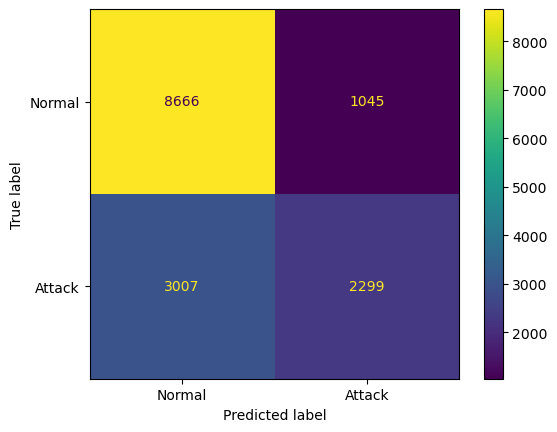
\includegraphics[width=0.7\linewidth]{files/2e2c6ebe209596e9ad0e5938a236242e.png}

\paragraph{Part 4 - Visualizing}

\subparagraph{Receiver Operating Characteristic (ROC) Curve and Area Under Curve (AUC)}

\begin{verbatim}
from sklearn.metrics import roc_curve, auc
import matplotlib.pyplot as plt

# Generate probabilities
y_pred_prob = classifier.predict(X_test).ravel()

# Calculate ROC curve
fpr, tpr, thresholds = roc_curve(y_test, y_pred_prob)
roc_auc = auc(fpr, tpr)

# Plot ROC curve
plt.figure()
plt.plot(fpr, tpr, label=f'ROC Curve (AUC = {roc_auc:.2f})')
plt.plot([0, 1], [0, 1], 'k - -')  # Random guess line
plt.xlabel('False Positive Rate')
plt.ylabel('True Positive Rate')
plt.title('Receiver Operating Characteristic')
plt.legend(loc='lower right')
plt.savefig('ROC_SA.png')
plt.show()
\end{verbatim}

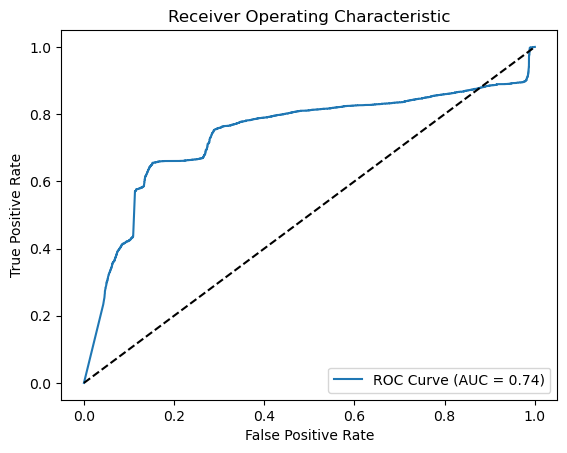
\includegraphics[width=0.7\linewidth]{files/e58b405eed076528e08019c85c6d53a5.png}

\subparagraph{Plot the accuracy}

\begin{verbatim}
########################################
# Part 4 - Visualizing
#######################################

# Import matplot lib libraries for plotting the figures. 
import matplotlib.pyplot as plt

# You can plot the accuracy
print('Plot the accuracy')
# Keras 2.2.4 recognizes 'acc' and 2.3.1 recognizes 'accuracy'
# use the command python -c 'import keras; print(keras.__version__)' on MAC or Linux to check Keras' version
plt.plot(classifierHistory.history['accuracy'], label='Training Accuracy')
#plt.plot(classifierHistory['accuracy'], label='Training Accuracy')
plt.title('model accuracy')
plt.ylabel('accuracy')
plt.xlabel('epoch')
plt.legend(loc='upper left')
plt.savefig('accuracy_sample_SA.png')
plt.show()
\end{verbatim}

\begin{verbatim}
Plot the accuracy
\end{verbatim}

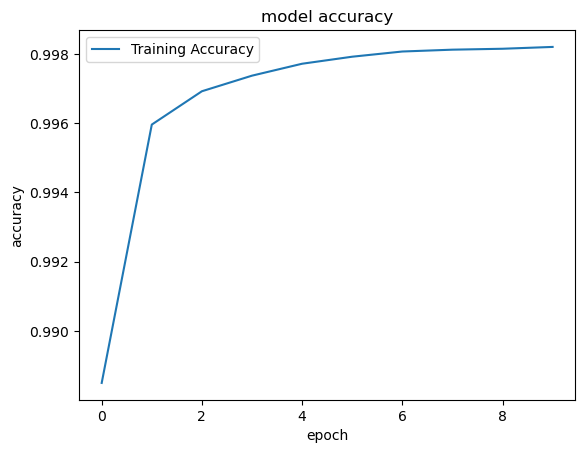
\includegraphics[width=0.7\linewidth]{files/8bf953608f9a63f08d9a86458d406a19.png}

\subparagraph{Plot the Loss}

\begin{verbatim}
# You can plot history for loss
print('Plot the loss')
plt.plot(classifierHistory.history['loss'], label='Training Loss')
#plt.plot(classifierHistory['loss'], label='Training Loss')
plt.title('model loss')
plt.ylabel('loss')
plt.xlabel('epoch')
plt.legend(loc='upper left')
plt.savefig('loss_sample_SA.png')
plt.show()
\end{verbatim}

\begin{verbatim}
Plot the loss
\end{verbatim}

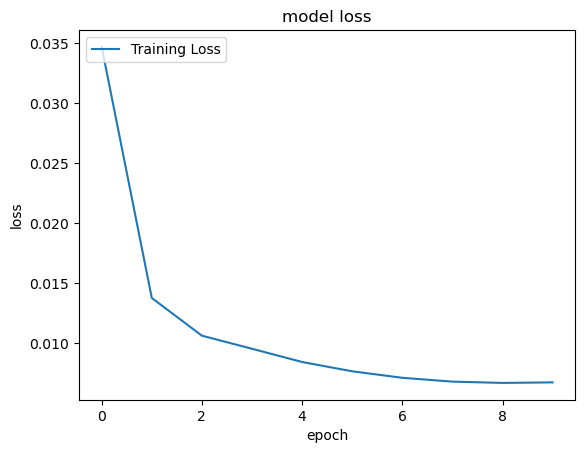
\includegraphics[width=0.7\linewidth]{files/8c03da1270e327d43cc7e6502b8b78e8.png}